%\documentclass[12pt, letterpaper, titlepage]{article}
\documentclass[12pt, letterpaper]{article}

\usepackage{amsmath, amsfonts}
\usepackage{booktabs}
\usepackage{amsthm}
\usepackage{graphicx}
\usepackage[margin=1in]{geometry}
\usepackage{hyperref}
\usepackage{cleveref}
\hypersetup{colorlinks = true, linkcolor = blue, citecolor=blue, urlcolor = blue}
\usepackage{natbib}
\usepackage{float}
\usepackage{setspace}
\usepackage{pdfpages}
\usepackage{lineno}
\usepackage{mwe}
\usepackage{comment}
\linenumbers*[1]
% %% patches to make lineno work better with amsmath
\newcommand*\patchAmsMathEnvironmentForLineno[1]{%
 \expandafter\let\csname old#1\expandafter\endcsname\csname #1\endcsname
 \expandafter\let\csname oldend#1\expandafter\endcsname\csname end#1\endcsname
 \renewenvironment{#1}%
 {\linenomath\csname old#1\endcsname}%
 {\csname oldend#1\endcsname\endlinenomath}}%
\newcommand*\patchBothAmsMathEnvironmentsForLineno[1]{%
 \patchAmsMathEnvironmentForLineno{#1}%
 \patchAmsMathEnvironmentForLineno{#1*}}%

\AtBeginDocument{%
 \patchBothAmsMathEnvironmentsForLineno{equation}%
 \patchBothAmsMathEnvironmentsForLineno{align}%
 \patchBothAmsMathEnvironmentsForLineno{flalign}%
 \patchBothAmsMathEnvironmentsForLineno{alignat}%
 \patchBothAmsMathEnvironmentsForLineno{gather}%
 \patchBothAmsMathEnvironmentsForLineno{multline}%
}

% control floats
\renewcommand\floatpagefraction{.9}
\renewcommand\topfraction{.9}
\renewcommand\bottomfraction{.9}
\renewcommand\textfraction{.1}
\setcounter{totalnumber}{50}
\setcounter{topnumber}{50}
\setcounter{bottomnumber}{50}

\newcommand{\jy}[1]{\textcolor{blue}{JY: #1}}
\newcommand{\eds}[1]{\textcolor{red}{EDS: (#1)}}
\newcommand{\of}[1]{\textcolor{violet}{OF: #1}}

% NOTE: To produce blinded version, replace "0" with "1" below.
\newcommand{\blind}{0}

%\title{On Devon Allen's Disqualification at the 2022 World Track and Field
%Championships}
%
%\author{Owen Fiore\\
%%   \href{mailto:owen.fiore@uconn.edu}
%% {\nolinkurl{owen.fiore@uconn.edu}}\\
  %Elizabeth D. Schifano\\
  %Jun Yan\\[1ex]
  %Department of Statistics, University of Connecticut\\
%}
%\date{}

\begin{document}

\title{\bf Supplement to ``On Devon Allen's Disqualification at the 2022 World Track and Field Championships''}

\if0\blind
{
  \author{Owen Fiore, %\\
%   \href{mailto:owen.fiore@uconn.edu}
% {\nolinkurl{owen.fiore@uconn.edu}}\\
  Elizabeth D. Schifano, %\\
  Jun Yan\\[1ex]
  Department of Statistics, University of Connecticut\\
}
} \fi

\if1\blind
{
  \bigskip
  \bigskip
  \bigskip
  \author{Anonymous Authors}
  \bigskip
} \fi

\maketitle 

\section{Rank-Based Comparison with Pooled Data}

\jy{Keep the order consistent with the text; do the same in the code.}

As an alternative to the methods described in Section 3.1 of the main paper, it
is possible to combine all men's and women's reaction time (RT) data for each of 
the three competition
comparisons.  Thus we shrink our analyses from six to three, but each analysis
is roughly twice as big as previously.  For the 2019 versus 2022 comparison,
there were 258 RTs from 65 athletes and the asymptotic
test result was a p-value of $3.56 \cdot 10^{-8}$. For the 2022 national versus
international comparison, there were 160 RTs from 35
athletes and the asymptotic test result was a p-value of $1.94 \cdot 10^{-7}$.
For the 2023 versus 2022 comparison, there were 343 RTs
from 92 athletes and the asymptotic test result was a p-value of
$4.99 \cdot 10^{-12}$.  These are all highly significant test results that show
substantial differences in average RT for athletes competing at
multiple championship-level events.


\section{GAMLSS Results for Women Data}

We can repeat our reaction time barrier analysis described in Section 3.2, but
fit the same model to women's RT data from 2001 to 2023.  Once again we utilize
the power of the venue effect within $\mu$ and a heat effect within $\sigma$.
\eds{what is meant by `power' here?} 
The RT data for women is visualized in Figure~\ref{fig:WomensBoxplot}.
Similar to the men's data, RTs from 2022 appear lower than in other
years.



\begin{figure}[tbp]
  \centering
  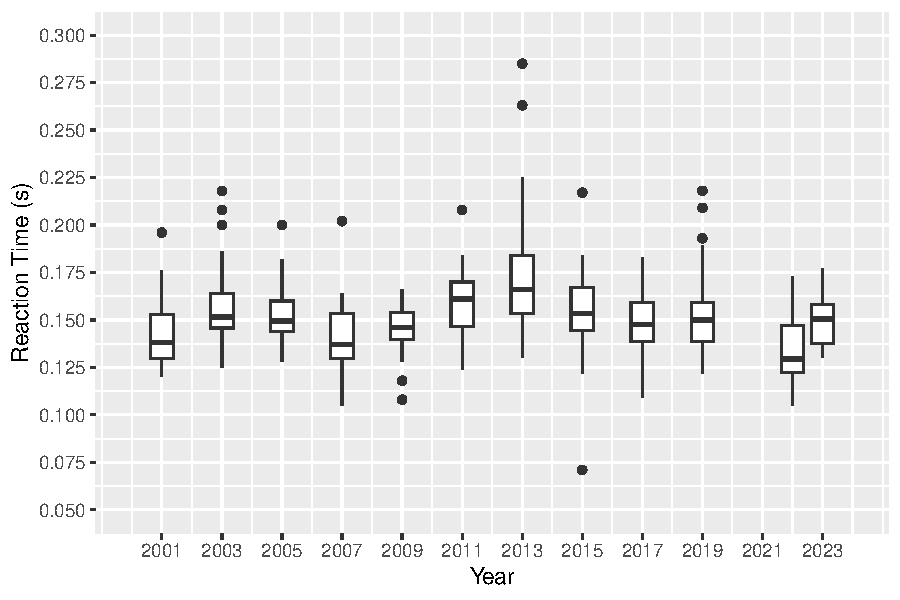
\includegraphics[width=\textwidth]{WomensBoxplot}
  \caption{The RTs from 2021 to 2023 for the women's 100 meter hurdle
  and 100 meter dash.}
  \label{fig:WomensBoxplot}
\end{figure}

The results are slightly different from those from the men's data,
which echoes existing studies reporting gender differences in RTs 
\citep[e.g.,][]{lipps2011implications, babicc2009reaction,
  panoutsakopoulos2020gender}.

\of{Currently cannot fit the gg3b to the men's and womens data}


\section{Results from Data Excluding Positive Disqualified RTs}

An earlier iteration of the paper fit a model that did not include RTs from
athletes who were disqualified or did not finish but still registered a RT.  
However, it was ultimately decided to include these times to better estimate the 
left tail of the distribution and more accurately predict the probability of a 
low RT, as described in the main paper.  
We did not include negative RTs, however, as these represent a mistake 
of the runner for starting before
the gun is fired and are thus meaningless in our objective to
determine a fair RT barrier.  Not all of those disqualified were
disqualified because of breaking the 0.1 reaction time barrier; there are many
reasons why an athlete may be disqualified, with the most notable being failed
drug tests and lane violations.  Nonetheless, in this section,
we exclude all disqualified RTs to see their effect on the probability of an
extreme RT.  We fit an identical model to the generalized Gamma model
presented in Section 3.2 to examine differences results.

\begin{table}
  \centering
  \caption{Probabilities of observing RTs less than threshold 0.08,
  0.09, and 0.10 seconds based on the
    fitted GG GAMLSS model with both venue- and heat-level
random effects.}
  \begin{tabular}{c c c c}
   \toprule
   Data Set & Threshold 0.08 & Threshold 0.09 & Threshold 0.10  \\
   \midrule
   Without DQs & $4.93\cdot10^{-5}$ & $3.53\cdot10^{-4}$ &  $1.97\cdot10^{-3}$  \\
   With DQs & $6.84\cdot10^{-5}$ & $4.95\cdot10^{-4}$ & $2.76\cdot10^{-3}$ \\
   \bottomrule
  \end{tabular}
  \label{tab:DQSim_probability}
\end{table}

\jy{Men's data or pooled data?}
\eds{with or without 2022?}

Table~\ref{tab:DQSim_probability} shows the effect of removing disqualificated
times from the analysis.  The probability of observing extreme RTs is lower when
we remove the 17 observations.

\bibliographystyle{apalike}
\bibliography{citations}


\end{document}
